% Molecular Modeling Lecture 6 LJ potential and integrators

\documentclass{beamer}

\mode<presentation>
{
%  \usetheme{Warsaw}
%\usetheme{Singapore}
%\usetheme{Dresden}
\usetheme{Hannover}
%\usetheme{Montpellier}
% nothing gives default

% Apparently these do nothing
%\usecolortheme{seahorse}
%\usecolortheme{rose}
\usepackage{beamerthemesplit} % new 
  \setbeamercovered{transparent}
  % or whatever (possibly just delete it)
}

\usepackage[english]{babel}
% or whatever

\usepackage[latin1]{inputenc}
% or whatever

\usepackage{times}
%\usepackage{auto-pst-pdf}
%\usepackage[T1]{fontenc}
% Or whatever. Note that the encoding and the font should match. If T1
% does not look nice, try deleting the line with the fontenc.

% Color text
\usepackage{xcolor}

\definecolor{olive}{rgb}{0.3, 0.4, .1}
\definecolor{fore}{RGB}{249,242,215}
\definecolor{back}{RGB}{51,51,51}
\definecolor{title}{RGB}{255,0,90}
\definecolor{dgreen}{rgb}{0.,0.6,0.}
\definecolor{gold}{rgb}{1.,0.84,0.}
\definecolor{JungleGreen}{cmyk}{0.99,0,0.52,0}
\definecolor{BlueGreen}{cmyk}{0.85,0,0.33,0}
\definecolor{RawSienna}{cmyk}{0,0.72,1,0.45}
\definecolor{Magenta}{cmyk}{0,1,0,0}


\title[Molecular Modeling and Simulation] % (optional, use only with long paper titles)
{CBE 60475/40475 Molecular Modeling and Simulation}
%\subtitle

\author[Marin, Shah and Maginn, Univ. of Notre Dame] % (optional, use only with lots of authors)
{E. Marin-Rimoldi, J.K. Shah \and  E. J.~Maginn}

%\author[(c) 2013, Maginn and Shah, Univ. of Notre Dame] % (optional, use only with lots of authors)
%{E. J.~Maginn, \and J.~Shah}

\institute[University of Notre Dame] % (optional, but mostly needed)
{
%  \inst{1}%
  Department of Chemical and Biomolecular Engineering\\
  University of Notre Dame \\
  Notre Dame, IN 46556 USA}
% - Use the \inst command only if there are several affiliations.

\date[September 9, 2013] % (optional, should be abbreviation of conference name)
{Cassandra Tutorial: Monte Carlo Simulation of Liquids}

\subject{Molecular Modeling and Simulation}
% This is only inserted into the PDF information catalog. Can be left
% out. 

% If you have a file called "university-logo-filename.xxx", where xxx
% is a graphic format that can be processed by latex or pdflatex,
% resp., then you can add a logo as follows:
%\pgfdeclareimage[height=0.5cm]{university-logo}{NDmark_small}
%\logo{\pgfuseimage{university-logo}}

% Add footnote to the bottom of each page
\setbeamertemplate{footline}[text line]{(c) 2013 University of Notre Dame} 

% Delete this, if you do not want the table of contents to pop up at
% the beginning of each subsection:
%\AtBeginSubsection[]
%{
%  \begin{frame}<beamer>{Outline}
%    \tableofcontents[currentsection,currentsubsection]
%  \end{frame}
%}
% If you wish to uncover everything in a step-wise fashion, uncomment
% the following command: 

%\beamerdefaultoverlayspecification{<+->}

% page numbers upper left
%\setbeamertemplate{headline}{\scriptsize{\vspace*{0.3cm}\hspace*{0.3cm}\insertframenumber}}

% This puts page number / total pages in bottom right corner
\setbeamertemplate{footline}[frame number]

\usepackage{times}
\def\boldpi{\mbox{\boldmath $\pi$}}
\def\boldrho{\mbox{\boldmath $\rho$}}
\def\boldPsi{\mbox{\boldmath $\Psi$}}

%---------------------------------------------------------
\begin{document}

\begin{frame}
  \titlepage
\end{frame}

%---------------------------------------------------------
\section{Cassandra Tutorial}
%---------------------------------------------------------
\begin{frame}{Simulation of Liquids in Cassandra}

Goal: Set up a MC simulation of Pentane from scratch.

\begin{itemize}
\item United Atom Model
\item TraPPE force field (Transferable Potentials for Phase Equilibria)
\item Features:
\begin{itemize}
	\item fixed bond lengths
	\item harmonic angle potentials
		\begin{equation}
			\nu_\theta = K_\theta(\theta-\theta_0)^2
		\end{equation}
	\item OPLS functional form for dihedral potentials
		\begin{equation}
                        \nu_\phi = \frac{1}{2}K_1[1+cos(\phi)]+\frac{1}{2}K_2[1-cos(2\phi)]
                \end{equation}
		\begin{equation}
\frac{1}{2}K_3[1+cos(3\phi)]+\frac{1}{2}K_4[1-cos(4\phi)]
		\end{equation}

\end{itemize}
\end{itemize}
\end{frame}
%---------------------------------------------------------
%\begin{frame}{Simulation of Liquids in Cassandra}

%\begin{figure}
%\begin{center}
%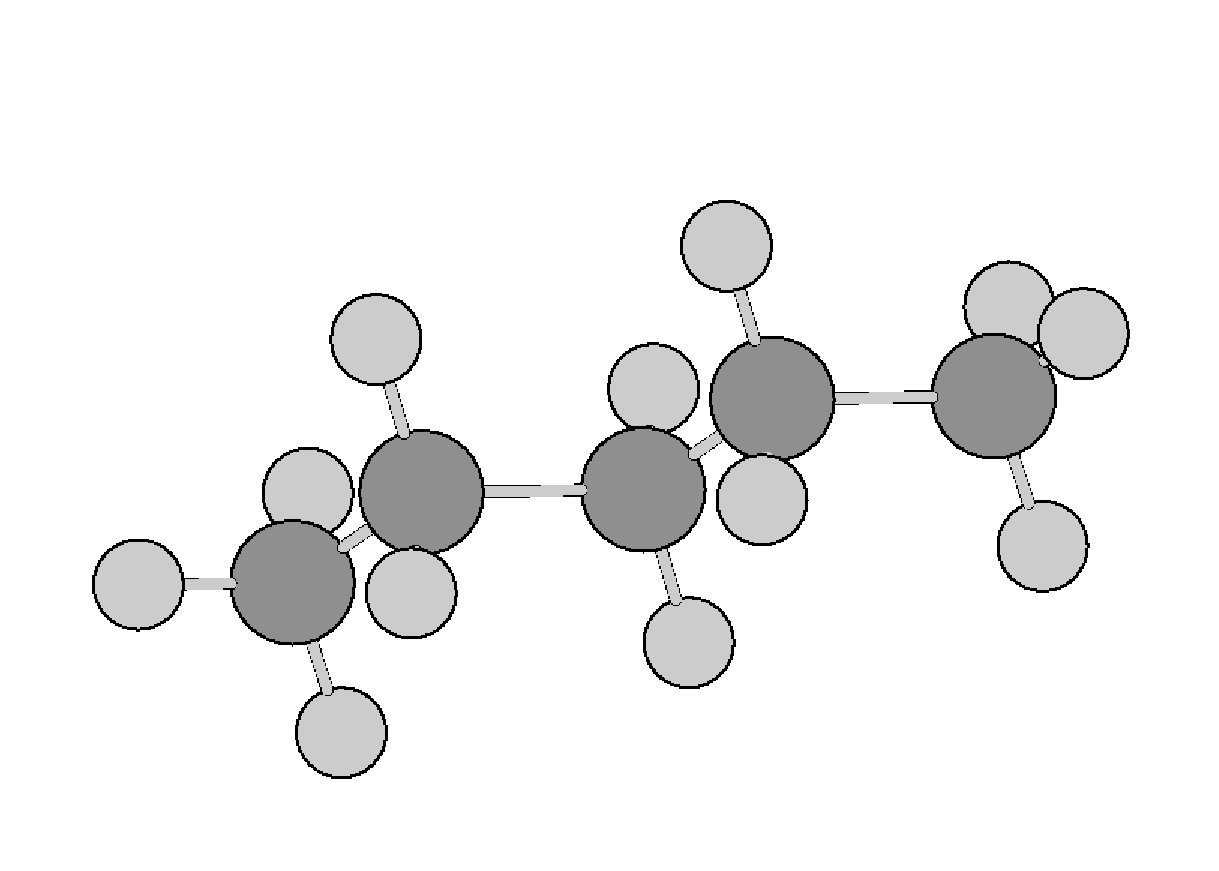
\includegraphics[height=1.3in]{pentaneAA.eps}
%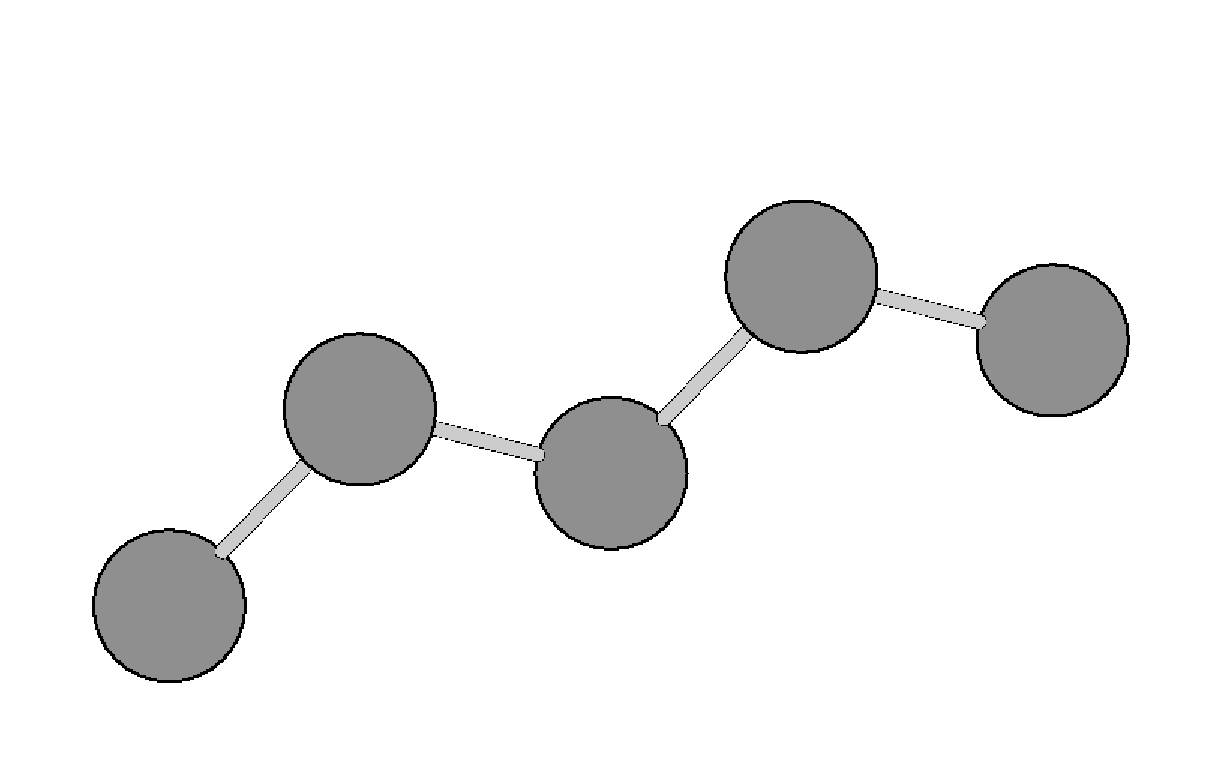
\includegraphics[height=1.3in]{pentaneUA.eps} \\
%United atom Pentane model.
%\end{center}
%\end{figure}

%\end{frame}
%---------------------------------------------------------
%\begin{frame}{Simulation of Liquids in Cassandra}

%\begin{figure}

%\begin{center}
%\includegraphics[height=2.0in]{flowsheet.eps}
%\end{center}
%Set up flowsheet of a Cassandra simulation
%\end{figure}

%\end{frame}
%---------------------------------------------------------


%\begin{frame}{Simulation of Liquids in Cassandra}

%\begin{figure}

%\begin{center}
%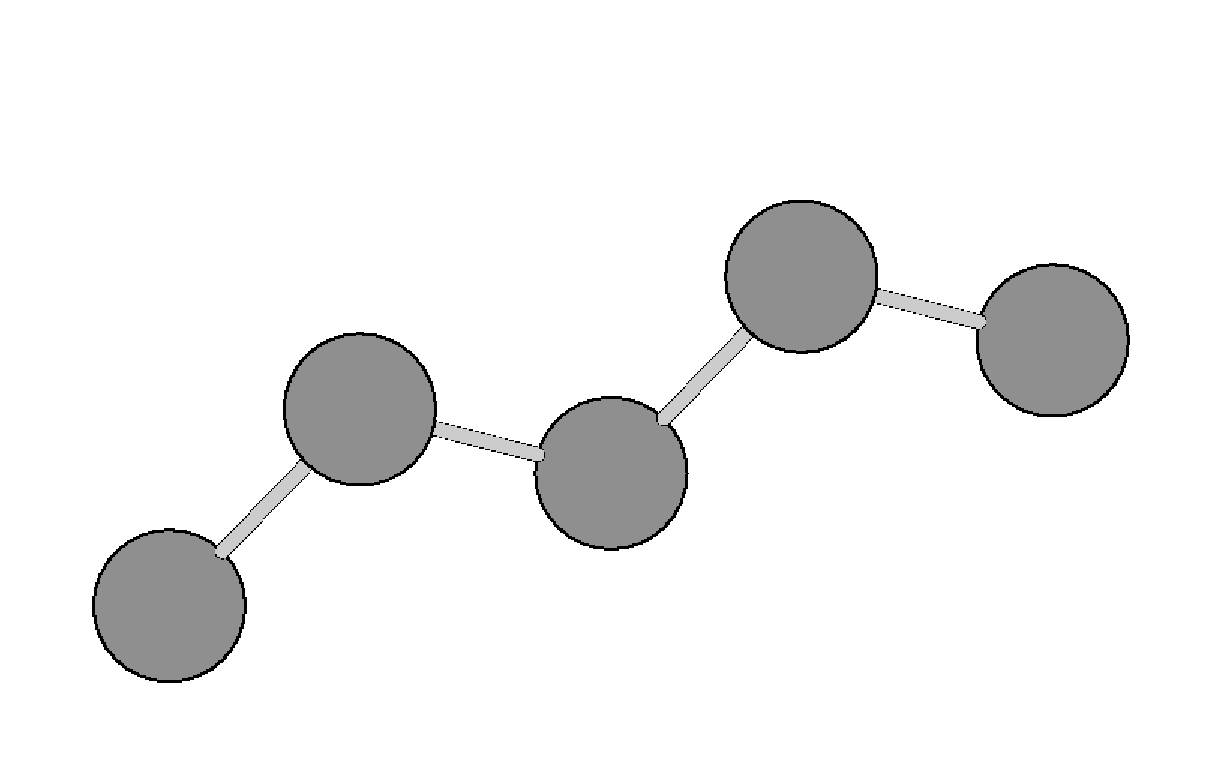
\includegraphics[height=2.0in]{pentaneUA.eps}
%\end{center}
%United atom Pentane
%\end{figure}

%\end{frame}
%---------------------------------------------------------

%\begin{frame}{Simulation of Liquids in Cassandra}

%\begin{figure}

%\begin{center}
%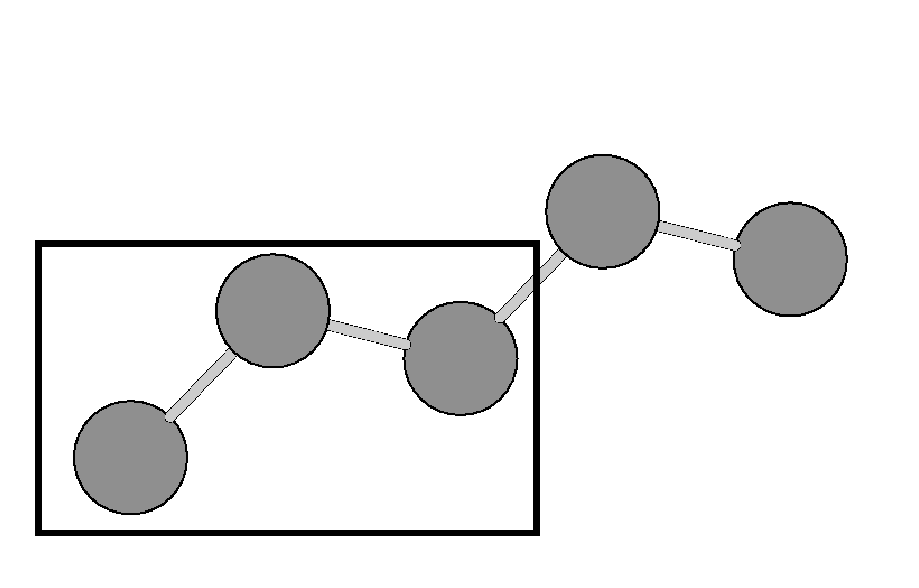
\includegraphics[height=2.0in]{pentaneUAfrag1.eps}
%\end{center}
%Fragment 1 pentane
%\end{figure}

%\end{frame}
%---------------------------------------------------------
%\begin{frame}{Simulation of Liquids in Cassandra}

%\begin{figure}

%\begin{center}
%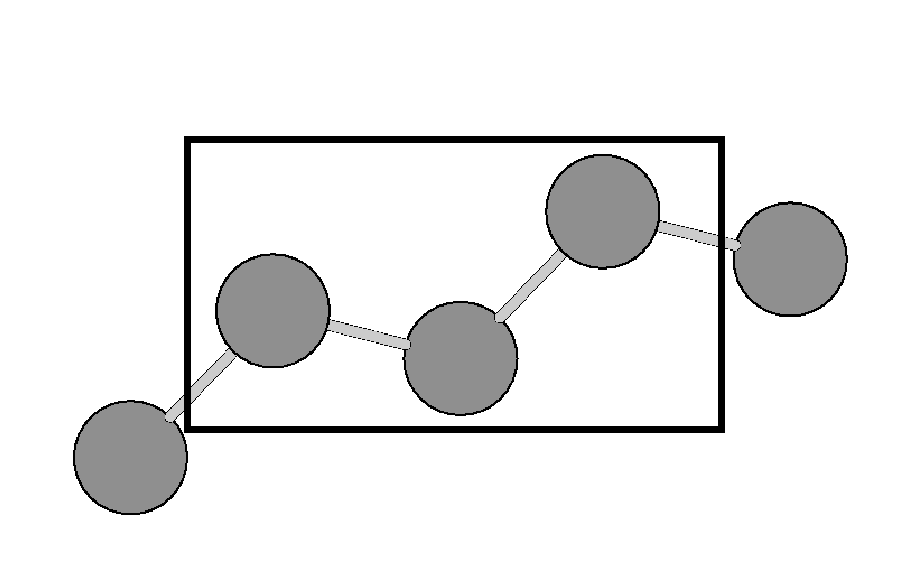
\includegraphics[height=2.0in]{pentaneUAfrag2.eps}
%\end{center}
%Fragment 2 pentane
%\end{figure}

%\end{frame}
%---------------------------------------------------------
%\begin{frame}{Simulation of Liquids in Cassandra}

%\begin{figure}

%\begin{center}
%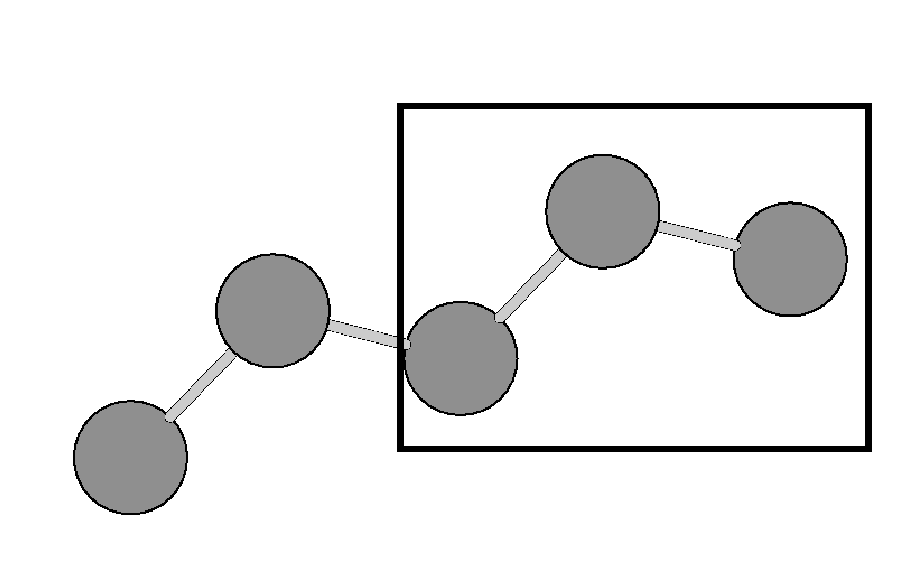
\includegraphics[height=2.0in]{pentaneUAfrag3.eps}
%\end{center}
%Fragment 3 pentane
%\end{figure}

%\end{frame}
%---------------------------------------------------------



\begin{frame}{Simulation of Liquids in Cassandra}

Motivation: Manual generation of MCF files can be error-prone for large molecules.
Automation tools: mcfgen.py.
Steps:
\begin{itemize}
	\item Obtain a PDB (protein data bank) file of the molecule
	\item Run: mcfgen.py -fffile molecule.pdb OR mcfgen.py -fffile molecule.cml
	\item Fill out the generated molecule.ff with the parameters found in literature
	\item Run: mcfgen.py -cassandra molecule.pdb. The script will assume molecule.ff
		is located in the current directory. 
	\item Check the generated mcf file (molecule.mcf)
	\item Generate fragment library by running library\_setup.py: library\_setup.py \$path/cassandra.exe inputfile.inp molecule1.pdb molecule2.pdb ...
\end{itemize}

\end{frame}
%---------------------------------------------------------
\begin{frame}{Obtaining a PDB file of the molecule}

Options:
\begin{itemize}
\item Obtain from databases (i.e. www.rcsb.org). 
\item Generate using drawing tools (i.e. Gaussview, Avogadro). 
\end{itemize}

Note that this script has been tested only with PDB files generated
by Gaussview 5.08 or Avogadro 1.1.1.

\end{frame}
%---------------------------------------------------------
\begin{frame}{Using Gaussview to generate a PDB file}
\begin{figure}
\begin{center}
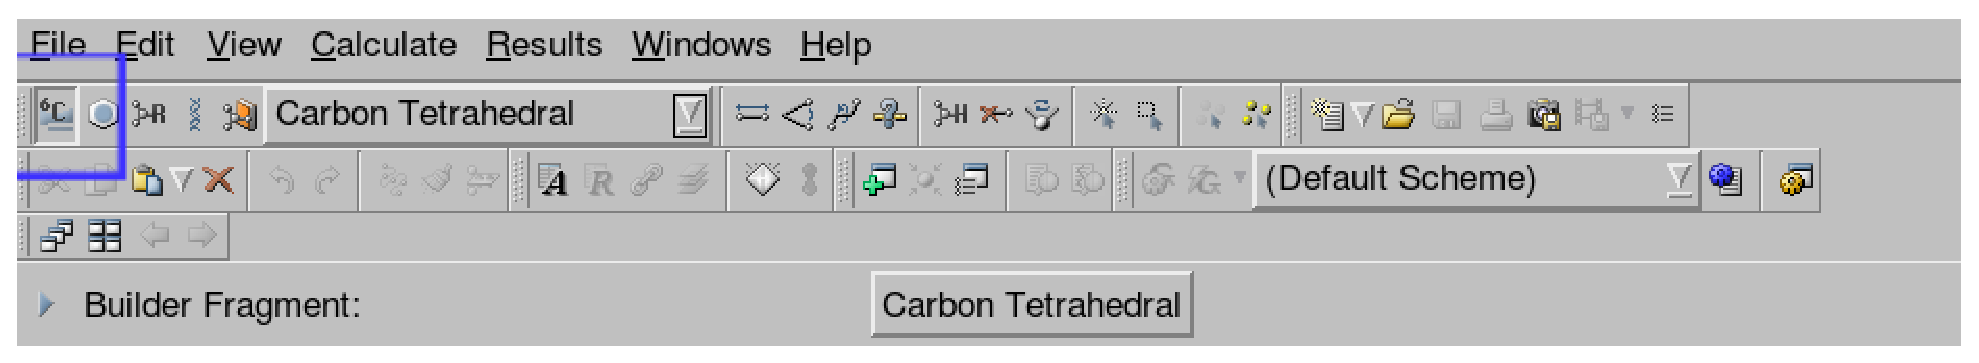
\includegraphics[height=1in]{gaussian1final.eps}
\end{center}
Click on the button "C" to display the periodic table
\end{figure}
\end{frame}
%---------------------------------------------------------
\begin{frame}{Using Gaussview to generate a PDB file}
\begin{figure}
\begin{center}
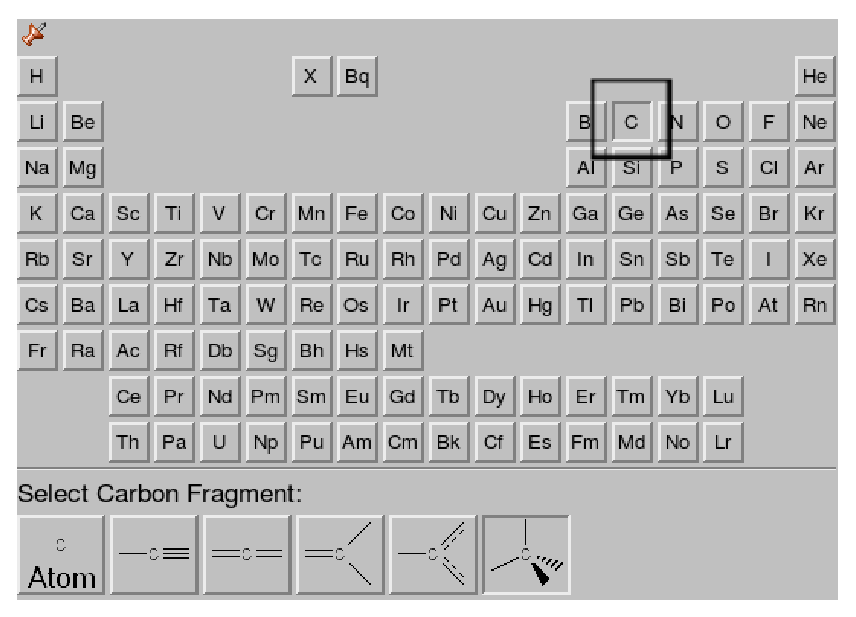
\includegraphics[height=3in]{gaussian2final.eps}
\end{center}
Click on "C" for Carbon
\end{figure}
\end{frame}
%---------------------------------------------------------
\begin{frame}{Using Gaussview to generate a PDB file}
\begin{figure}
\begin{center}
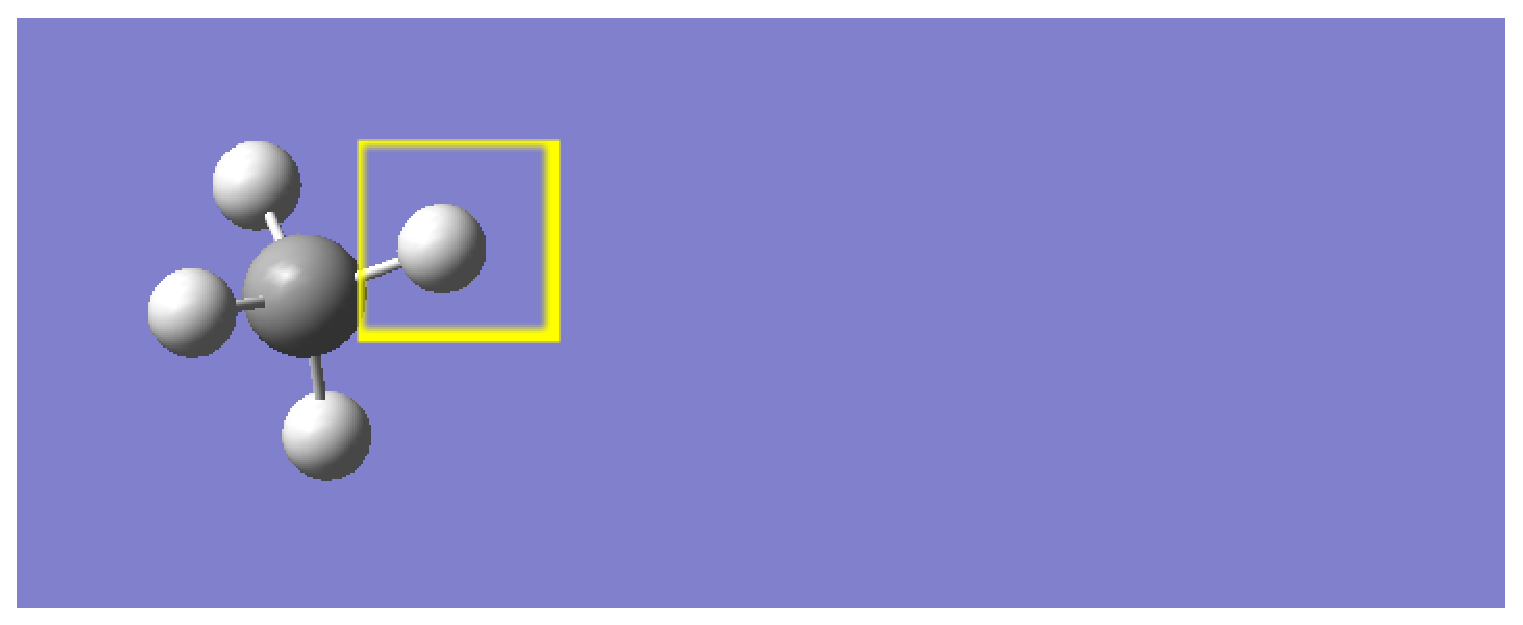
\includegraphics[height=2in]{gaussian3final.eps}
\end{center}
Click on the purple workplace to insert the first $CH_4$ fragment. 
To increase the chain length, click on a Hydrogen attached to the 
Carbon.
\end{figure}
\end{frame}
%---------------------------------------------------------
\begin{frame}{Using Gaussview to generate a PDB file}
\begin{figure}
\begin{center}
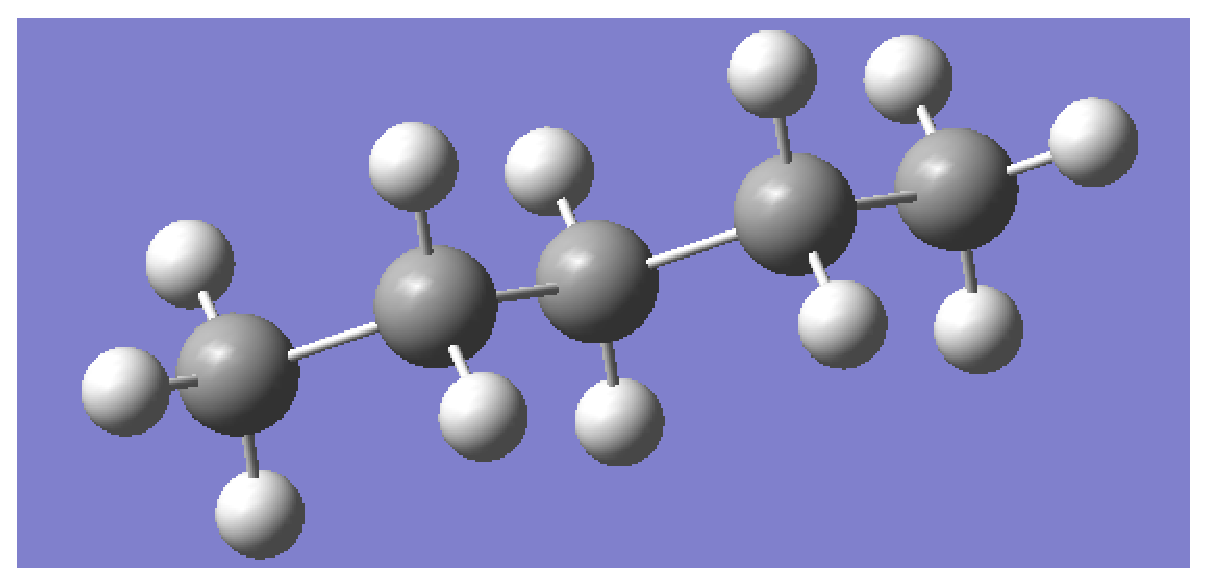
\includegraphics[height=2in]{gaussian4final.eps}
\end{center}
\end{figure}
\end{frame}
%---------------------------------------------------------
\begin{frame}{Using Gaussview to generate a PDB file}
\begin{figure}
\begin{center}
\includegraphics[height=2.5in]{gaussian5final.eps}
\end{center}
Right Click - Builder - Delete Atoms
\end{figure}
\end{frame}
%---------------------------------------------------------
\begin{frame}{Using Gaussview to generate a PDB file}
\begin{figure}
\begin{center}
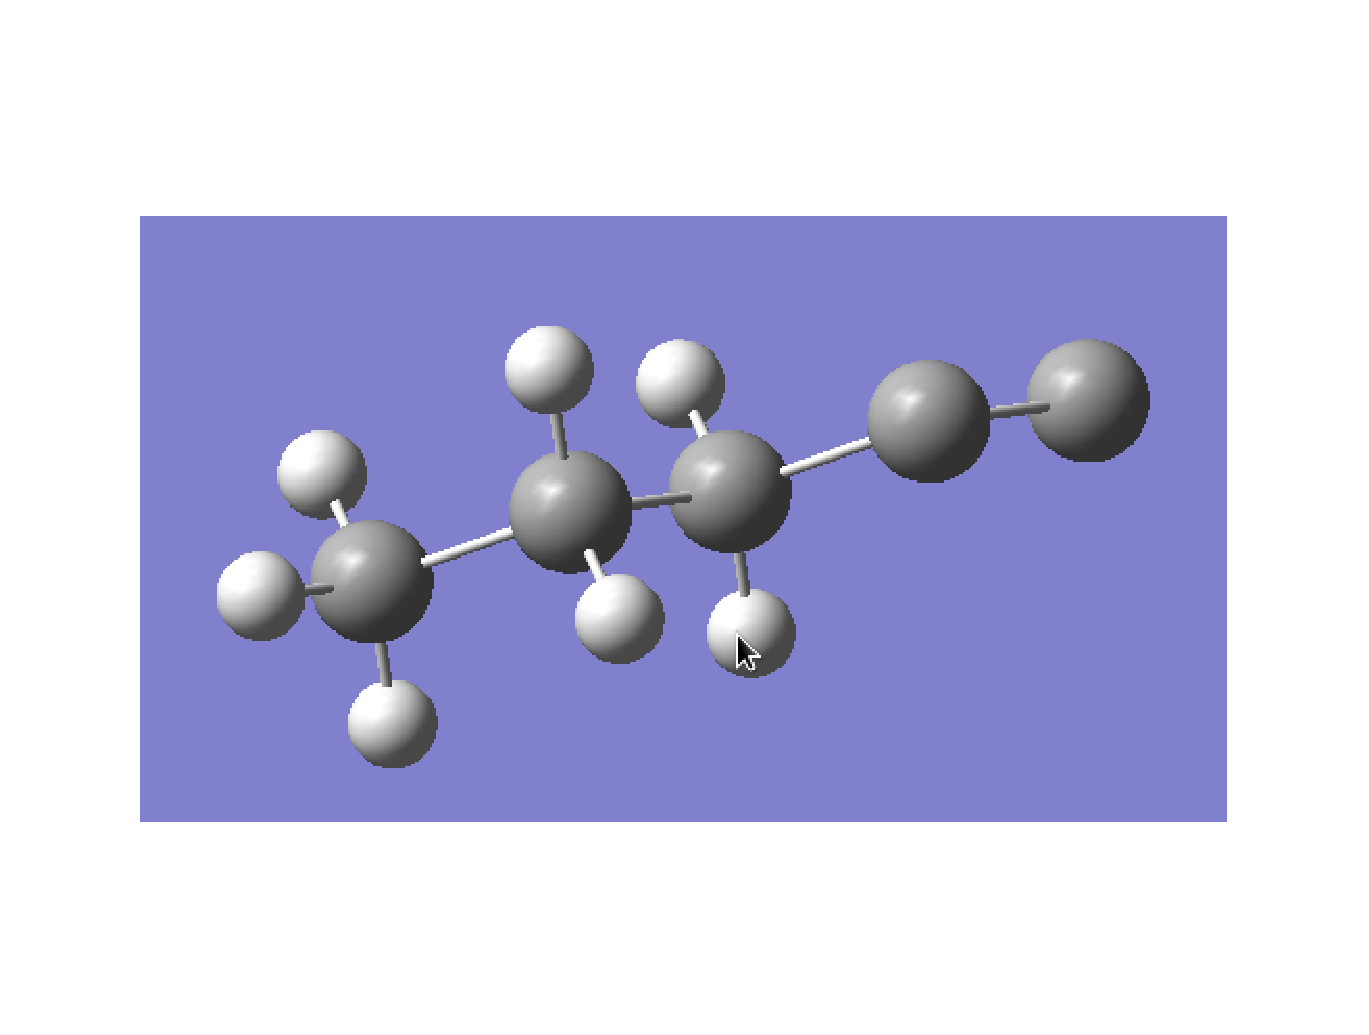
\includegraphics[height=2.5in]{gaussian7final.eps}
\end{center}
Click on Hydrogen atoms to delete them
\end{figure}
\end{frame}
%---------------------------------------------------------
\begin{frame}{Using Gaussview to generate a PDB file}
\begin{figure}
\begin{center}
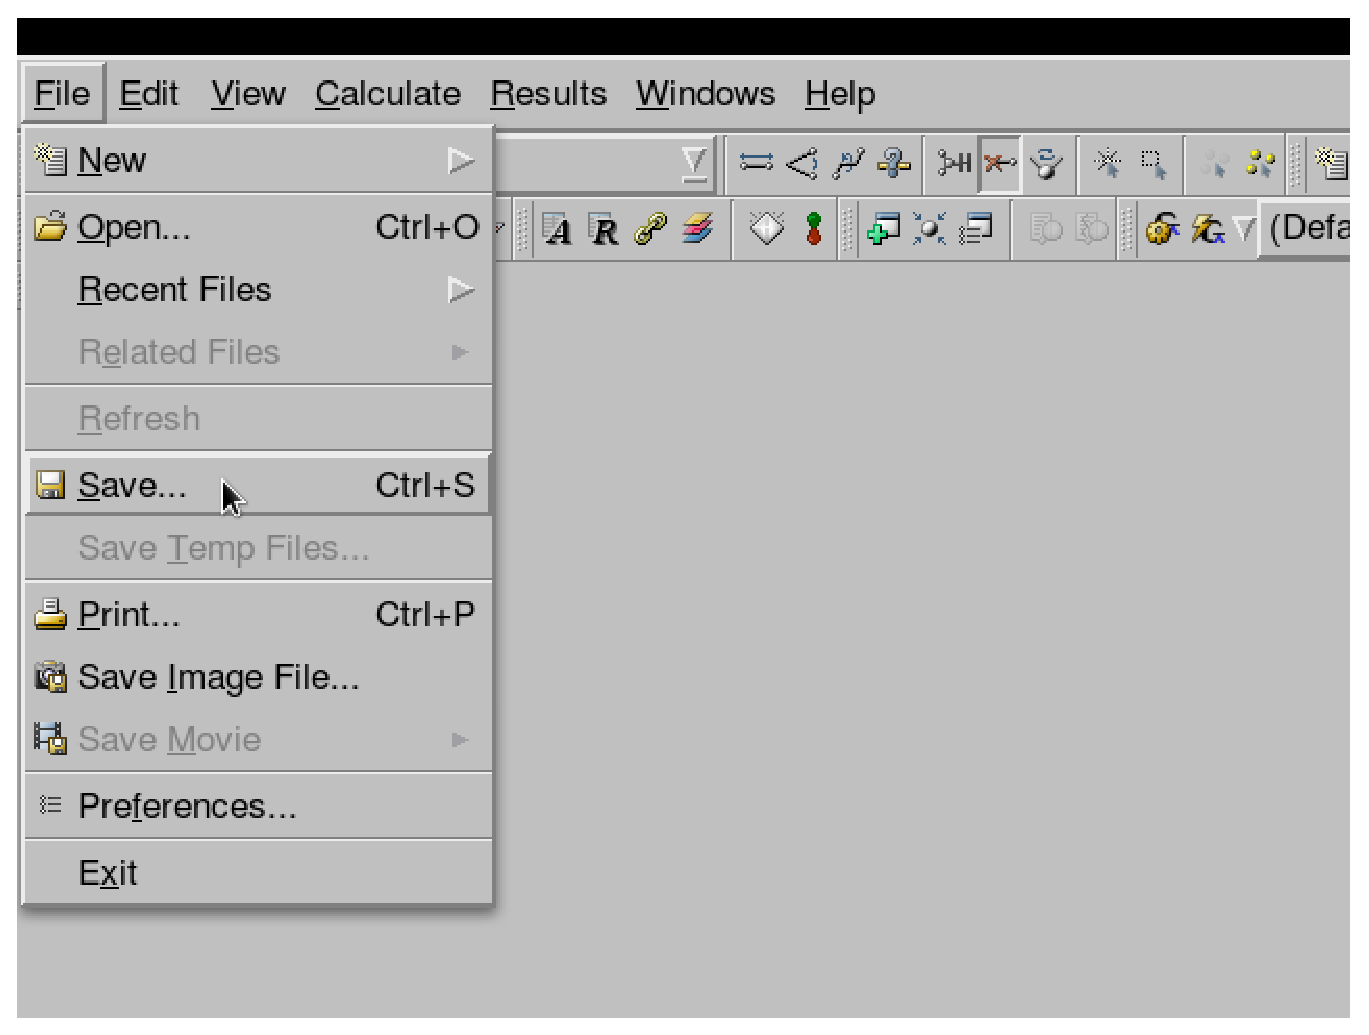
\includegraphics[height=2.5in]{gaussian8final.eps}
\end{center}
Go back to main menu. File - Save
\end{figure}
\end{frame}
%---------------------------------------------------------
\begin{frame}{Using Gaussview to generate a PDB file}
\begin{figure}
\begin{center}
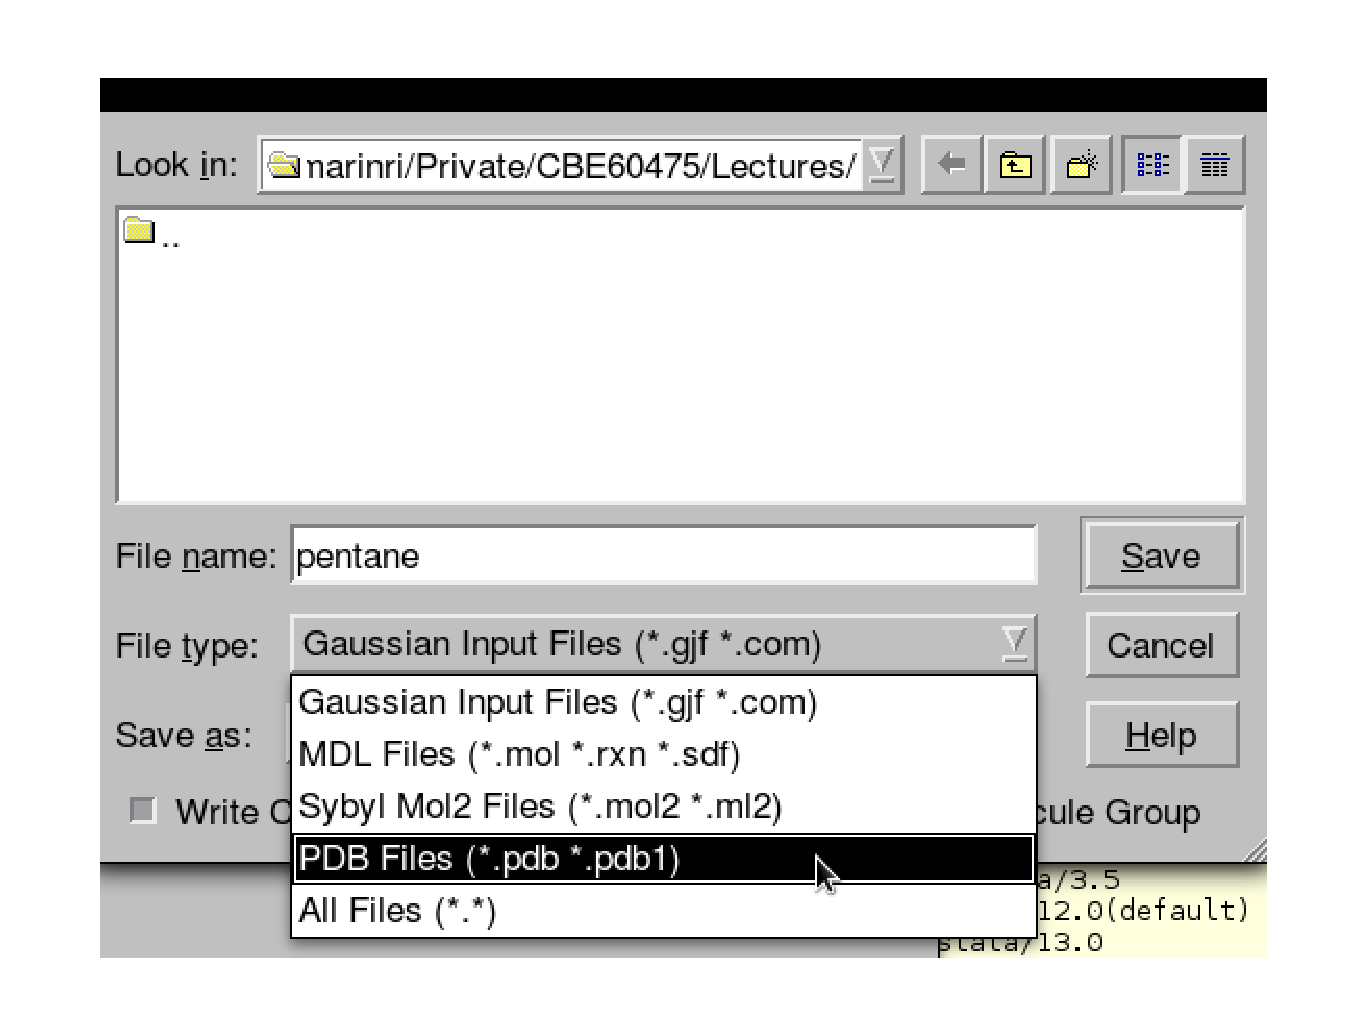
\includegraphics[height=2.5in]{gaussian9final.eps}
\end{center}
Type the name of the file. Select PDB file from the bottom menu.
\end{figure}
\end{frame}
%---------------------------------------------------------
\begin{frame}{Using Gaussview to generate a PDB file}
\begin{figure}
\begin{center}
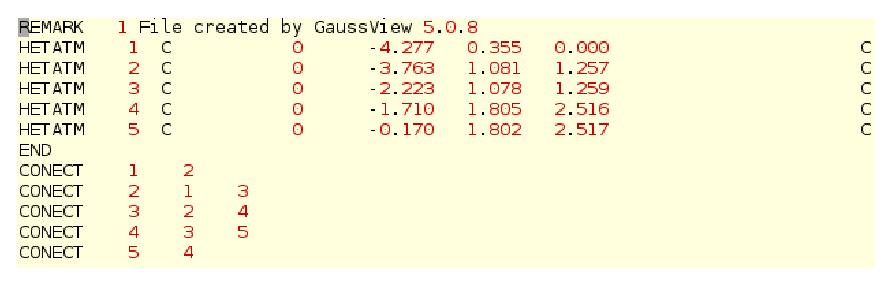
\includegraphics[height=1in]{pdbfile_final.eps}
\end{center}
Close Gaussview. Back in the terminal, Open the PDB File using your favorite text editor.
\end{figure}
\end{frame}
%---------------------------------------------------------
\begin{frame}{Using Gaussview to generate a PDB file}
\begin{figure}
\begin{center}
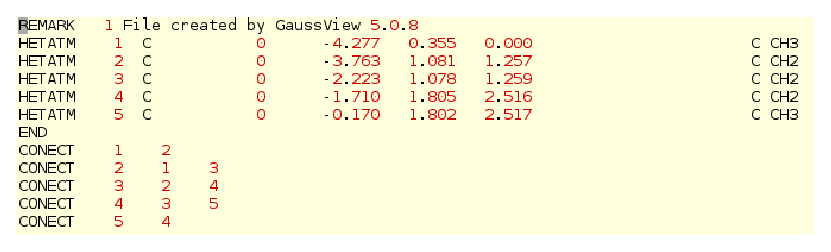
\includegraphics[height=1in]{pdbfile_edited_final.eps}
\end{center}
Append a column containing the atom types.
\end{figure}
\end{frame}
%---------------------------------------------------------
\begin{frame}{Using Avogadro to generate a CML file}
Avogadro can be used to generate CML files. The procedure is analogous to the one previously
presented for Gaussview.
\end{frame}
%---------------------------------------------------------
\begin{frame}{Using Avogadro to generate a CML file}
\begin{figure}
\begin{center}
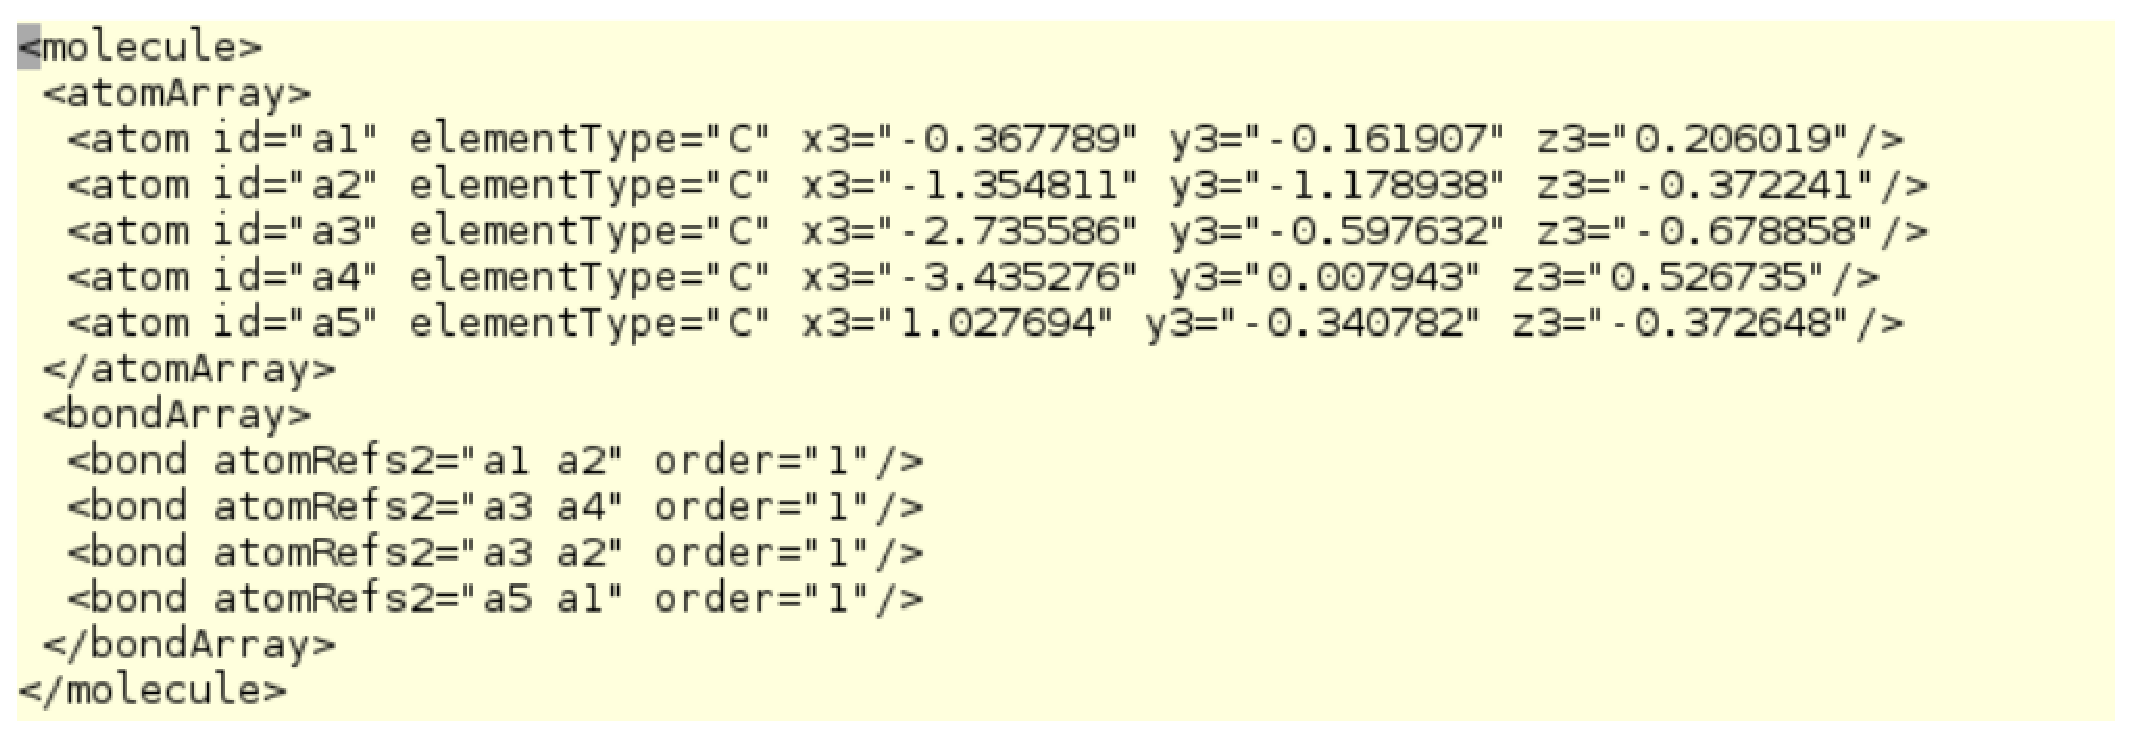
\includegraphics[height=1in]{pentane_cml.eps}
\end{center}
Pentane united atom CML file generated using Avogadro
\end{figure}
\end{frame}
%---------------------------------------------------------
\begin{frame}{Using Avogadro to generate a CML file}
\begin{figure}
\begin{center}
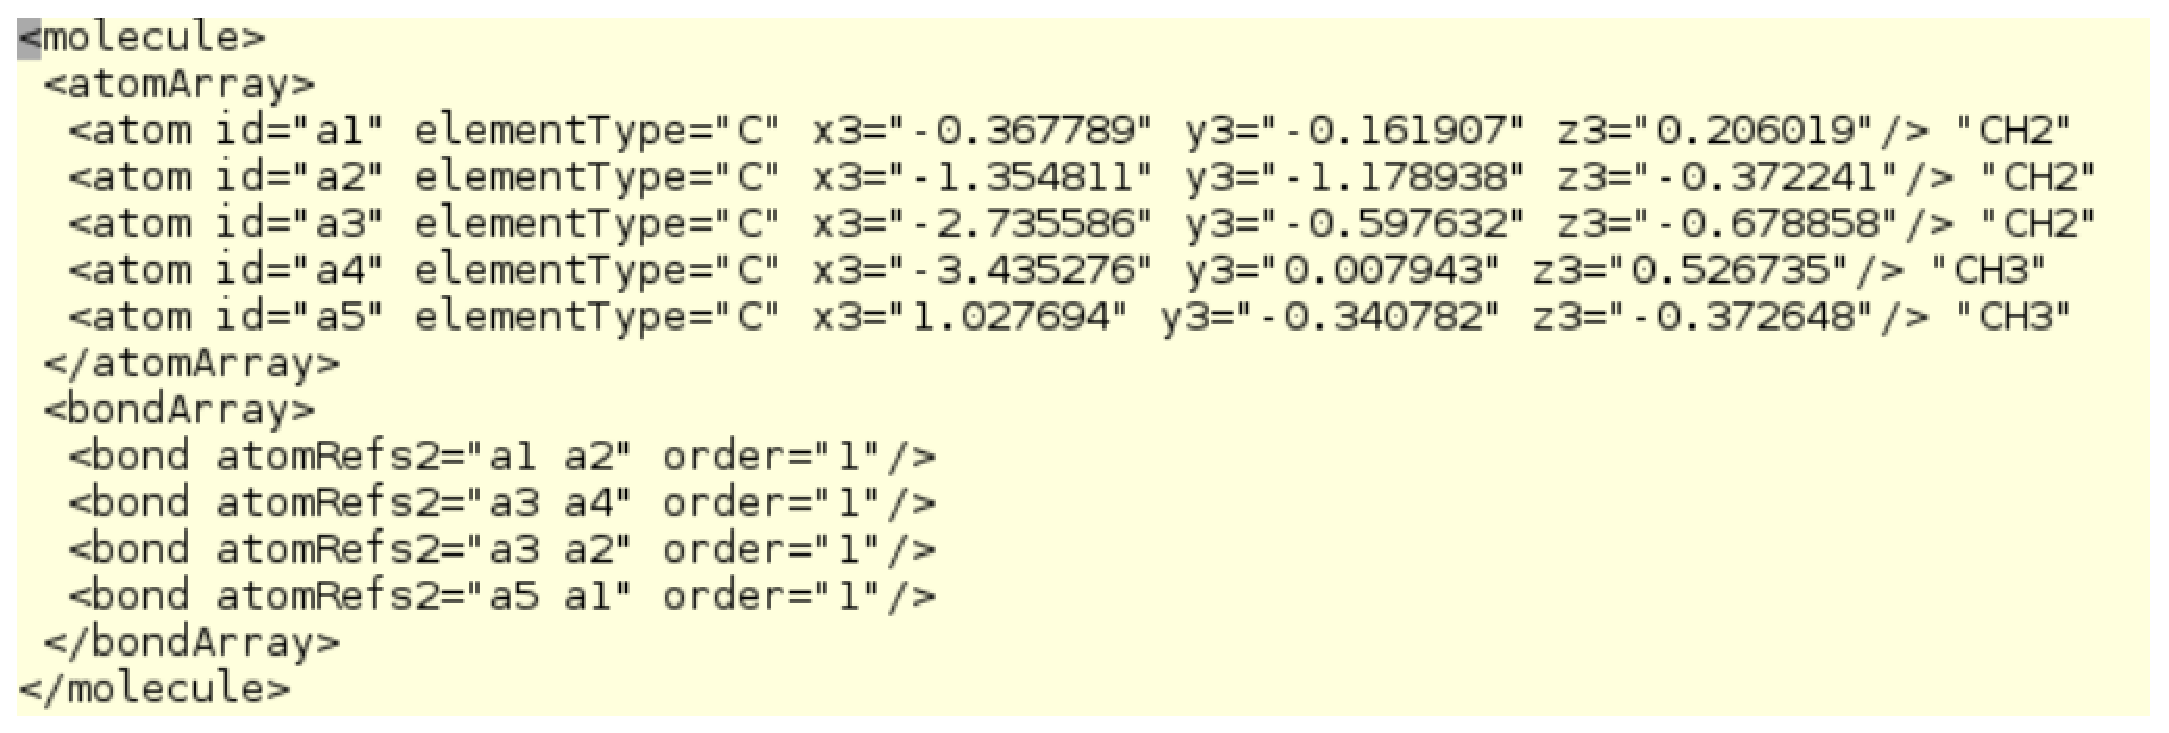
\includegraphics[height=1in]{pentane_cml_modified.eps}
\end{center}
Modified pentane united atom CML file. Note the atom type is appended as a last column between quotation marks.
\end{figure}
\end{frame}
%---------------------------------------------------------
\begin{frame}
\begin{itemize}
\item Run the following command:
\end{itemize}
\texttt{> module load python} \\
\texttt{> python mcfgen.py -fffile pentane.pdb}
\begin{itemize}
\item Fill out the newly created .ff file with literature values (see next slide).
\end{itemize}
\end{frame}
%---------------------------------------------------------
\begin{frame}
\begin{figure}
\begin{center}
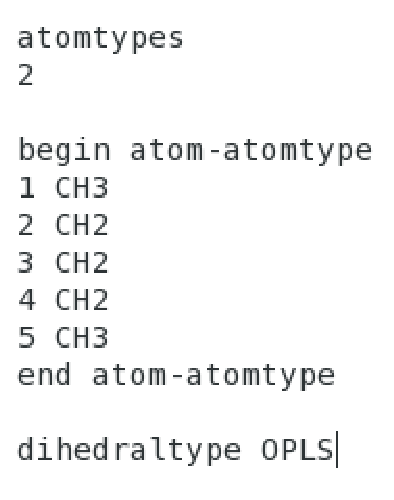
\includegraphics[height=1in]{top_ff.eps}
\end{center}
The first three sections of the FF file are displayed above. Do not modify these.
\end{figure}

\end{frame}
%---------------------------------------------------------
\begin{frame}
\begin{figure}
\begin{center}
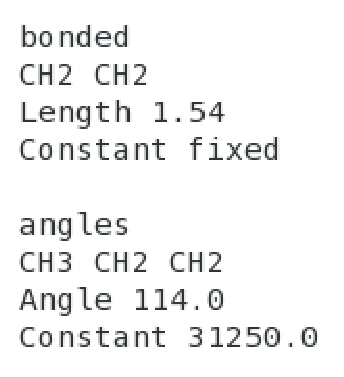
\includegraphics[height=1in]{body_ff.eps}
\end{center}
The force field parameters for non-bonded (not shown), bonded, angle, dihedral (not shown) and coulombic interactions (not shown) must be entered next to the corresponding keyword. For example, the angle type CH3 CH2 CH2 has an angle of 114.0. This value must be placed next to the `Angle' keyword.
\end{figure}

\end{frame}

%---------------------------------------------------------

\begin{frame}
For more examples of filled FF files, please refer to the examples contained in the /Scripts/ directory.
\end{frame}

%---------------------------------------------------------
\begin{frame}
\begin{itemize}
\item Using the filled .ff file, run:
\end{itemize}
\texttt{>  python mcfgen.py -cassandra pentane.pdb}
\begin{itemize}
\item Check the file pentane.mcf for any possible errors.
\item Substitute pentane.pdb by pentane.cml if CML files are being used.
\item Note that the FF file must be in the same current directory as the PDB or CML file.
\end{itemize}
\end{frame}
%---------------------------------------------------------
\begin{frame}
\begin{itemize}
\item Prepare an input file, specifying the ensemble to be used, box lengths, probabilities, etc...
\item To set up the simulation, run:
\end{itemize}
\texttt{> python library\_setup.py inputfile.inp species1.pdb species2.pdb}
\\
Note that the script library\_setup.py will assume that the PDB files, MCF files and input file
are in the same current directory.

\begin{itemize}
\item To run the simulation:
\end{itemize}
\texttt{> \$path/cassandra.exe inputfile.inp}
\end{frame}
%---------------------------------------------------------
\begin{frame}
Things to take care:
\begin{itemize}
\item Units and force field functional forms must be consistent with those required by Cassandra. See documentation for further information.
\item Manually change molecular weights for United Atom models in the MCF file (i.e. CH$_3$ has a weight of 15 g/mol instead of 12 g/mol)
\item Some software generate PDB/CML files with a format that this script does not recognize. Please check the provided examples to see how a PDB should look like.
\item This script does not recognize byciclic molecules (e.g. decalin).
\end{itemize}
\end{frame}
%---------------------------------------------------------
\begin{frame}{Flowsheet}
\begin{figure}
\begin{center}
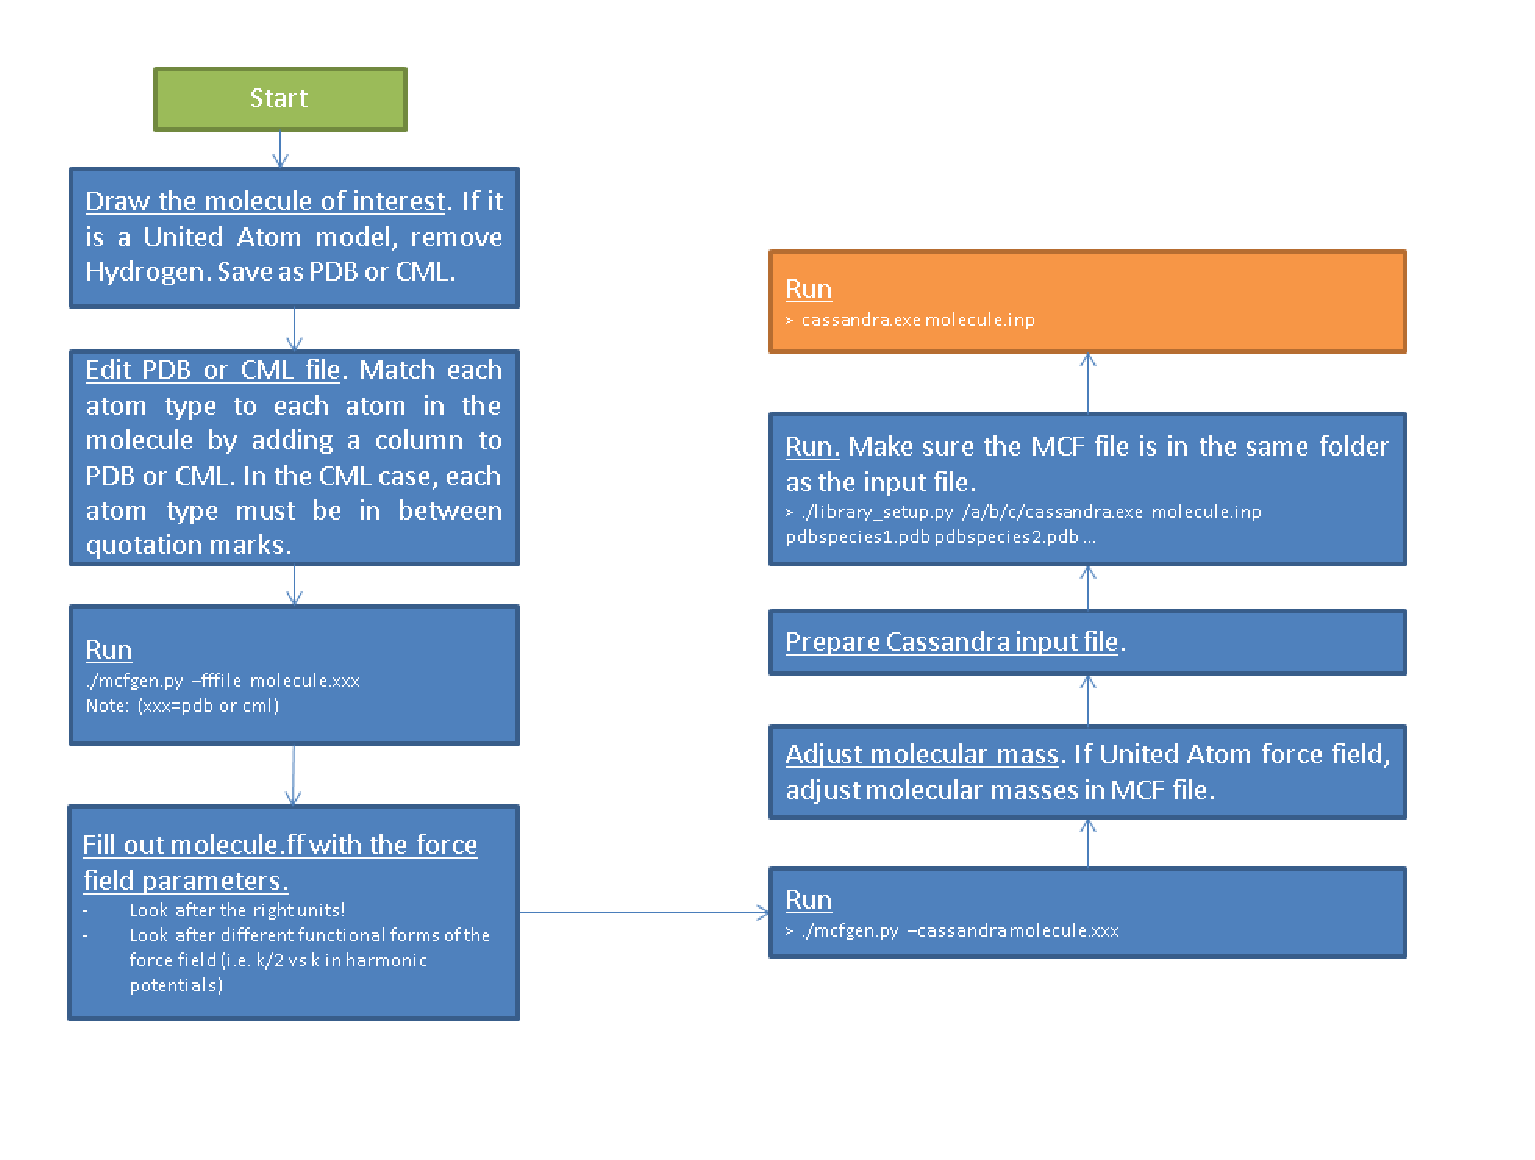
\includegraphics[height=3in]{simulationsetup_betarelease.eps}
\end{center}
\end{figure}
\end{frame}



\end{document}
